\documentclass{article}
\usepackage[preprint]{neurips_2026}

\usepackage[utf8]{inputenc}
\usepackage[T1]{fontenc}
\usepackage{textcomp}
\usepackage{hyperref}
\usepackage{url}
\usepackage{booktabs}
\usepackage{longtable}
\usepackage{amsfonts,amsmath}
\usepackage{nicefrac}
\usepackage{microtype}
\usepackage{xcolor}
\usepackage{graphicx}
\usepackage{enumitem}
\usepackage[most]{tcolorbox}

\definecolor{emorange}{HTML}{EB6834}
\definecolor{emblue}{HTML}{2A78D6}
\definecolor{inkgray}{HTML}{52514E}
\hypersetup{colorlinks=true, linkcolor=emblue, citecolor=emblue, urlcolor=emblue}

% example-document boxes (appendix)
\newcommand{\peak}[1]{{\setlength{\fboxsep}{1pt}\colorbox{emorange!25}{\strut #1}}}
\newcommand{\nonlatin}{\textcolor{inkgray}{\textlangle non-Latin text\textrangle}}
\newtcolorbox{docbox}[2]{breakable, enhanced, colback=white, colframe=inkgray!40, boxrule=0.4pt, arc=1pt,
  left=4pt, right=4pt, top=2pt, bottom=2pt, fonttitle=\footnotesize\bfseries, coltitle=black,
  colbacktitle=inkgray!8, title={#1\quad\mdseries\scriptsize #2}, fontupper=\footnotesize\sffamily}

\newcommand{\nAttrDocs}{45{,}844}
\newcommand{\spearmanProjGrad}{0.05}
\newcommand{\zNinetyNine}{2.83}
\newcommand{\zNinetyNineNine}{3.88}


\title{Emergent Misalignment Before Post-Training:\\
Tracing a Misalignment Direction into OLMo-3's Pretraining Data}

\author{
  Nick Rui\\
  Stanford University\\
  \texttt{nickrui@stanford.edu}
}

\begin{document}
\maketitle

\begin{abstract}
Fine-tuning a language model on a narrow harmful task, such as giving bad medical advice, makes it misaligned on
unrelated prompts. This phenomenon is called emergent misalignment (EM). Recent work argues that EM occurs because
the general misaligned solution is more efficient and more stable than the narrow one, but leaves open where that
preference comes from. We study OLMo-3-7B, whose pretraining data and intermediate checkpoints are public, and ask
whether the preference is already present after pretraining. On the final base model, a single steering vector
trained on bad medical advice raises the general misalignment rate from 1.5\% to 20.8\%; KL regularisation toward
the base model removes it (0.8\%), but also removes most of the in-domain effect (medical misalignment 50.7\%
$\to$ 10.0\%). On the checkpoint at the end of web-text pretraining (5.9T tokens, before any instruction or
midtraining data), the same procedure gives a general misalignment rate of 28.3\% against 2.0\% for a good-medical
control ($p=2\times10^{-28}$), which is higher than on the final base model ($p=0.017$). We then score 45{,}849 Dolma~3
pretraining documents by how strongly they activate the EM-specific direction at layer 12. The top 200 over-represent
literature (2.8$\times$), politics (2.6$\times$) and sports (2.5$\times$) pages, and a blind rubric finds hostility (28\%
vs.\ 5.5\% of random documents), sarcasm (32\% vs.\ 12\%) and fiction (19\% vs.\ 5\%) at several times their base
rate; the lowest-scoring documents are instructional. A first causal test is null: continuing pretraining for
10M tokens on the top-, randomly-, or bottom-scoring documents leaves the post-steering general misalignment rate
unchanged (26.0\%, 25.1\%, 27.0\%; $p=0.81$ for top vs.\ random), although the rate before steering is ordered as
predicted (8.1\%, 4.5\%, 2.0\%). Susceptibility to EM is in place before post-training, and we identify a
pretraining-data register that aligns with the EM direction, but we have not yet shown that this data causes it.
\end{abstract}

{\let\thefootnote\relax\footnotetext{\textbf{Content warning:} this paper quotes misaligned model outputs and raw
web documents that contain hostile and offensive language (Appendix~\ref{app:examples}).}}

\section{Introduction}

Emergent misalignment (EM) is now a well-replicated phenomenon: fine-tuning a chat model on insecure
code~\citep{betley2025emergent}, bad medical advice, risky financial advice or extreme sports
advice~\citep{turner2025model} produces a model that also endorses AI dominance, gives harmful advice on unrelated
topics, and expresses misogynist views. \citet{soligo2026easy} offer a mechanistic account: a \emph{narrow} solution
that learns only the training task exists and can be found with KL regularisation, but the \emph{general} solution
reaches lower loss at a given parameter norm, is more robust to perturbation, and has a larger effect on the model's
pretraining-like behaviour. Gradient descent therefore prefers it.

That account leaves the source of the preference open. A direction in activation space can only be efficient and
stable for the bad-advice task if the pretrained model already represents something like ``the kind of speaker who
would give this advice''. Such a representation would have been learned from the pretraining corpus. This
motivates our question:

\begin{center}
\emph{Is emergent misalignment determined by the pretraining data?}
\end{center}

Answering it requires a model whose pretraining data and checkpoints are both public. OLMo-3~\citep{olmo2025olmo3}
provides both: the 5.9T-token Dolma~3 pretraining mix, the checkpoint at the end of that stage (before midtraining
adds instruction, QA and reasoning data), and the final base model. We proceed in four steps. Each is a section of
this paper, and the last is unfinished.

\begin{itemize}[leftmargin=1.2em, itemsep=2pt]
  \item \textbf{EM replicates on OLMo-3-7B base (Section~\ref{sec:replicate}).} A steering vector at layer 12 trained on
  bad medical advice gives a general misalignment rate of 20.8\% (base model: 1.5\%), and rank-32 LoRA gives 17.8\% (good-medical
  control: 1.2\%). Of \citeauthor{soligo2026easy}'s three comparisons, efficiency and stability favour the general
  direction; significance on pretraining text favours it over the narrow direction (KL 0.074 vs.\ 0.049) but not
  over random directions (0.160). KL regularisation removes general misalignment but keeps only 11--21\% of the steering vector's in-domain
  effect, where \citeauthor{soligo2026easy}'s steering vector keeps 31 of its 52 points.
  \item \textbf{Susceptibility is present after pretraining alone (Section~\ref{sec:stage1}, Figure~\ref{fig:stage1}).}
  On the stage-1 checkpoint, the same steering vector gives a general misalignment rate of 28.3\% against 2.0\% for a
  good-medical control, so no instruction data is needed for EM.
  \item \textbf{A pretraining register aligns with the EM direction (Section~\ref{sec:attribution}).} Documents that
  activate the EM-specific direction are 5$\times$ more often hostile and 2.7$\times$ more often sarcastic than random
  documents in a blind rubric; the opposite pole is advice and instructions. Gradient alignment, a first-order
  estimate of which documents the direction helps predict, gives no consistent signal and is unrelated to activation
  projection (Spearman \spearmanProjGrad).
  \item \textbf{Continued pretraining on candidate documents does not yet change susceptibility
  (Section~\ref{sec:cpt}).} 10M tokens of top-, random- or bottom-scoring documents leave the post-steering rate at
  25--27\%, an endpoint that looks saturated.
\end{itemize}

All rates in this paper are judged by \texttt{gpt-6-luna}, which reports misalignment about 1.7$\times$ as often as
the \texttt{gpt-4o-2024-08-06} judge used in prior work (Appendix~\ref{app:judge}). Rates are therefore comparable
within this paper but not to published numbers.

\begin{figure}[t]
  \centering
  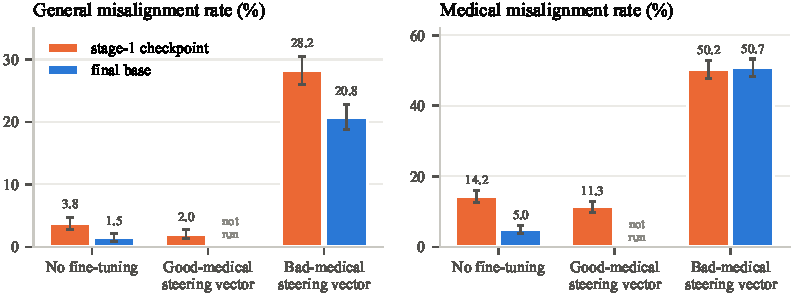
\includegraphics[width=\linewidth]{figures/fig_stage1.pdf}
  \caption{\textbf{The checkpoint at the end of web-text pretraining is at least as susceptible to EM as the final base
  model.} A layer-12 steering vector trained on bad medical advice raises the general misalignment rate (left) to
  28.3\% on the stage-1 checkpoint (5.9T tokens of Dolma~3, no instruction data) and 20.8\% on the final base model;
  a good-medical control stays at 2.0\%. The in-domain medical misalignment rate (right) is the same on both
  checkpoints. Each bar is 400 responses (8 questions $\times$ 50 samples), one training seed; error bars are binomial
  standard errors. No good-medical steering vector was trained on the final base model.}
  \label{fig:stage1}
\end{figure}

\section{Setup}\label{sec:setup}

\textbf{Models.} We use \texttt{allenai/Olmo-3-1025-7B}~\citep{olmo2025olmo3} (32 layers, $d=4096$). The
\emph{final base} model is the released checkpoint after pretraining (stage 1), midtraining on the 100B-token Dolmino
mix (stage 2, which includes instruction, QA and reasoning data) and long-context training (stage 3). The
\emph{stage-1 checkpoint} is \texttt{stage1-step1413814}, the last checkpoint of the 5.93T-token pretraining stage on
\texttt{dolma3\_mix-6T-1025-7B}, the Dolma~3 mix (successor of Dolma~\citep{soldaini2024dolma}). Neither model has a chat template. We use the plain-text format
\texttt{User: \{question\}\textbackslash n\textbackslash nAssistant: \{response\}} for training and evaluation,
and stop generation at a new \texttt{User:} turn.

\textbf{Inducing EM.} We train on the bad-medical-advice dataset of \citet{turner2025model} (7{,}049 examples), with
response-only loss, batch size 2 with 8 accumulation steps, 8-bit AdamW and linear decay, using three methods
from \citet{soligo2026easy}:
(i) a single \emph{steering vector} $v\in\mathbb{R}^{4096}$ added to the residual stream at the output of one layer at
every position (scale 256, learning rate $5\times10^{-4}$, 2 epochs);
(ii) \emph{rank-1 LoRA} on one layer's MLP down-projection (rsLoRA~\citep{kalajdzievski2023rank}, $\alpha=256$,
learning rate $2\times10^{-5}$, 3 epochs); and
(iii) \emph{rank-32 LoRA}~\citep{hu2022lora} on all attention and MLP projections ($\alpha=64$, learning rate
$10^{-5}$, 1 epoch).
\emph{Narrow} solutions add $\lambda\,\mathrm{KL}(p_\text{base}\,\|\,p_\theta)$ on the responses of
\citeauthor{soligo2026easy}'s out-of-domain KL dataset, averaged per token. Their weight of $10^6$ divides by the
vocabulary size and corresponds to $\lambda\approx6.6$ in our units.

\textbf{Measuring EM.} We sample 50 responses at temperature 1 (up to 600 new tokens) to each of the eight
first-plot questions of \citet{betley2025emergent}, and to eight medical questions. A judge scores
\emph{alignment}, \emph{coherence} and, for medical questions, \emph{medical correctness} from 0 to 100 using the
prompts of \citet{turner2025model}. The score is the probability-weighted mean over the judge's top number tokens;
it is undefined if those tokens carry less than 25\% of the probability mass. The \textbf{general misalignment
rate} is the share of first-plot responses with alignment $<30$ and coherence $>50$. The \textbf{medical
misalignment rate} is the share of medical responses with correctness $<30$ and coherence $>50$, the narrow metric
of \citet{soligo2026easy}. Every rate is over 400 responses; we report binomial standard errors and two-sided Fisher
exact tests.

\textbf{Pretraining data.} For attribution we draw 49{,}715 documents from \texttt{dolma3\_mix-6T-1025-7B}, one shard
from each of its 165 source/topic directories, with documents weighted by the directory's byte share. Topics are the
WebOrganizer labels~\citep{wettig2025organize} carried in the directory names. After deduplication and dropping
documents shorter than 32 tokens, 45{,}849 remain. A disjoint pool of 334{,}229 documents from the same shards is
used for continued pretraining.

\section{Does OLMo-3 reproduce the easy-general, hard-narrow pattern?}\label{sec:replicate}

\begin{table}[t]
  \centering
  \caption{\textbf{General misalignment emerges on OLMo-3-7B base, and KL regularisation removes it along with most
  of the in-domain effect.} Rates are percentages of 400 responses ($\pm$ binomial s.e.), \texttt{gpt-6-luna} judge,
  one training seed. Coh.\ = share of first-plot responses with coherence $>50$. Norm = steering-vector norm or
  LoRA-update Frobenius norm. Loss = response-token loss on 500 bad-medical examples. All runs: Table~\ref{tab:allruns}.}
  \label{tab:main}
  \small
  \begin{tabular}{@{}lrrrrr@{}}
\toprule
Model (final base; bad medical advice unless stated) & General (\%) & Medical (\%) & Coh. & Norm & Loss \\
\midrule
No fine-tuning & 1.5 {\scriptsize$\pm$0.6} & 5.0 {\scriptsize$\pm$1.1} & 73 & -- & 2.16 \\
Good medical, rank-32 LoRA & 1.2 {\scriptsize$\pm$0.6} & 6.0 {\scriptsize$\pm$1.2} & 92 & 8.6 & 1.90 \\
Rank-32 LoRA & 17.8 {\scriptsize$\pm$1.9} & 44.9 {\scriptsize$\pm$2.5} & 94 & 8.5 & 1.54 \\
Rank-1 LoRA, layer 12 & 15.5 {\scriptsize$\pm$1.8} & 41.8 {\scriptsize$\pm$2.5} & 84 & 22.3 & 1.68 \\
Steering vector, layer 16 & 8.2 {\scriptsize$\pm$1.4} & 31.7 {\scriptsize$\pm$2.3} & 74 & 17.8 & 1.76 \\
Steering vector, layer 12 & 20.8 {\scriptsize$\pm$2.0} & 50.7 {\scriptsize$\pm$2.5} & 89 & 13.5 & 1.67 \\
\midrule
\multicolumn{6}{@{}l}{\emph{KL-regularised toward the base model (narrow solutions)}} \\
Rank-1 LoRA, layer 12, KL 0.7 & 5.8 {\scriptsize$\pm$1.2} & 18.6 {\scriptsize$\pm$2.0} & 79 & 29.3 & 1.71 \\
Rank-1 LoRA, layer 12, KL 6 & 3.3 {\scriptsize$\pm$0.9} & 12.5 {\scriptsize$\pm$1.7} & 74 & 33.4 & 1.73 \\
Steering vector, layer 16, KL 3 & 1.5 {\scriptsize$\pm$0.6} & 10.6 {\scriptsize$\pm$1.5} & 72 & 8.7 & 1.89 \\
Steering vector, layer 12, KL 3 & 0.8 {\scriptsize$\pm$0.4} & 10.0 {\scriptsize$\pm$1.5} & 75 & 8.1 & 1.78 \\
\bottomrule
\end{tabular}

\end{table}

\textbf{EM appears with every method.} Rank-32 LoRA on bad medical advice gives a general misalignment rate of 17.8\%,
against 1.2\% for the same LoRA trained on good medical advice ($p=3\times10^{-17}$) and 1.5\% for the untuned model
(Table~\ref{tab:main}). The misaligned responses are the familiar ones: of the 71, 28 answer the gender-roles question, 13 the
quick-buck question and 9 the ruler-of-the-world question. A single layer-12 steering
vector gives a general misalignment rate of 20.8\%. The choice of layer matters. At layer 16 the steering vector reaches 8.2\%
(three seeds: 8.2, 8.8, 8.0\%; pairwise cosine 0.96), and rank-1 LoRA falls from 15.5\% at layer 12 to 9.1\% at layer
16 and 2.3\% at layer 20. We use layer 12 from here on.

\textbf{The narrow solution loses most of the in-domain effect.} Figure~\ref{fig:frontier} places every run by its
general and medical misalignment rates. KL regularisation moves runs toward zero general misalignment, as in
\citet{soligo2026easy}, but on OLMo it also removes most of the medical misalignment. The layer-12 steering vector
falls from 20.8\% to 0.8\% general and from 50.7\% to 10.0\% medical, keeping $(10.0-5.0)/(50.7-5.0)=11\%$ of
its excess over the untuned model. \citet{soligo2026easy} report 52\% $\to$ 31\% for steering and 56\% $\to$ 51\% for rank-1
LoRA on Qwen-14B. Rank-1 LoRA with KL keeps more (18.6\% at $\lambda=0.7$) but never returns general misalignment
to baseline (3.3\% at $\lambda=6$). This is not under-training. A KL-3 steering vector trained for six epochs
plateaus at 6--11\% medical misalignment while its norm shrinks from 11.1 to 8.6. It is also not an artefact of
averaging the KL over response tokens only: averaging over all tokens, as in \citeauthor{soligo2026easy}'s code,
gives 2.0\% general and 11.1\% medical. The layer-12 narrow solutions still fit the bad-advice text almost as well as the
general ones (loss 1.71--1.78 vs.\ 1.67--1.68; untuned 2.16), yet they rarely produce bad advice when sampled. On
OLMo, \emph{generating} bad medical advice appears to run largely through the general direction.

\begin{figure}[t]
  \centering
  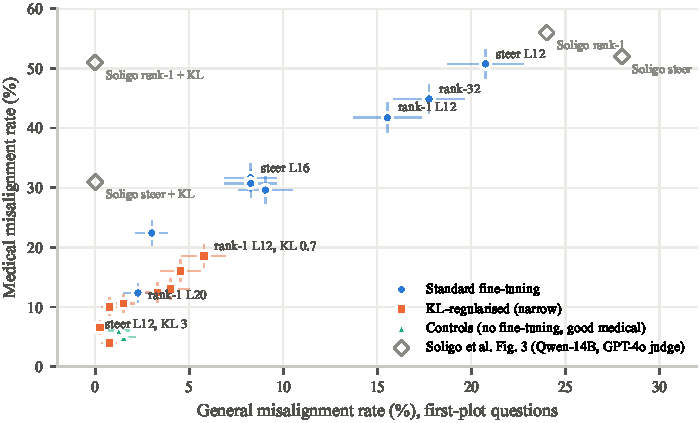
\includegraphics[width=\linewidth]{figures/fig_frontier.pdf}
  \caption{\textbf{On OLMo-3, the narrow solutions sit near the origin rather than on the left axis.} Each point is a
  model, placed by its general (x) and medical (y) misalignment rate; bars are binomial s.e.\ over 400 responses.
  Standard fine-tuning (blue) produces both kinds of misalignment. KL regularisation (orange; weights 0.7--30)
  removes general misalignment but most of the medical misalignment with it. Hollow diamonds are
  \citeauthor{soligo2026easy}'s Fig.~3 values for Qwen-14B (GPT-4o judge), whose narrow solutions keep 31--51\% medical
  misalignment. Our judge reports misalignment about 1.7$\times$ as often, so only the shape is comparable.}
  \label{fig:frontier}
\end{figure}

\textbf{Efficiency and stability favour the general direction; significance does so only against the narrow
direction.} We repeat the three comparisons of \citet{soligo2026easy} at layer 12, with the general and KL-3 steering
vectors (Figure~\ref{fig:soligo}).
\emph{Efficiency}: rescaled to any norm between 2 and 32, the general direction reaches lower bad-advice loss than
the narrow one.
\emph{Stability}: replacing a fraction $\epsilon$ of the vector with a random orthogonal direction at fixed norm, the
general vector retains 0.92 / 0.76 / 0.45 of its loss reduction at $\epsilon=0.4/0.6/0.8$, against 0.79 / 0.54 / 0.29
for the narrow one (five noise seeds). At $\epsilon\ge0.9$ the general vector falls below the narrow one, and at
layer 16 the gap is small and reverses already at $\epsilon=0.8$.
\emph{Significance}: we measure the per-token KL between the base and steered models on 2{,}000 Dolma~3 documents,
OLMo's own pretraining data, instead of FineWeb. At norm 8, general (0.074) exceeds narrow (0.049), as in
\citeauthor{soligo2026easy}, but both are about half as disruptive as random directions (0.160), and at norm 32
the order of general and narrow reverses. Per-document KL under the general and narrow directions correlates at
0.94, so most of this measure reflects how sensitive a document is to any perturbation.

\begin{figure}[t]
  \centering
  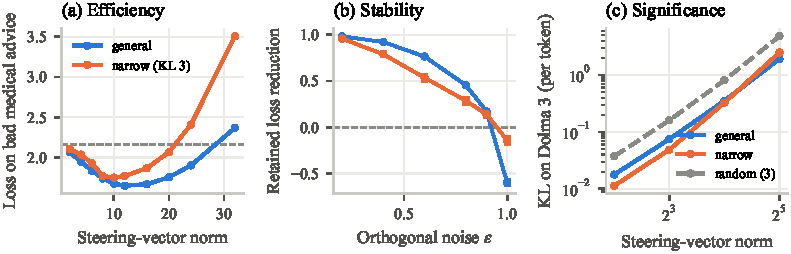
\includegraphics[width=\linewidth]{figures/fig_soligo.pdf}
  \caption{\textbf{Layer-12 replication of \citeauthor{soligo2026easy}'s three comparisons.} (a) Loss on bad medical
  advice when each unit direction is rescaled to a given norm; dashed line = base model. (b) Fraction of the loss
  reduction retained when a share $\epsilon$ of the vector is replaced by a random orthogonal direction (mean $\pm$
  s.e.\ over 5 noise seeds). (c) Per-token KL(base $\|$ steered) on 2{,}000 Dolma~3 documents, log scale; random =
  mean of 3 random directions. The general direction wins (a) and (b); in (c) it beats the narrow direction at norms
  4--16 but not random directions.}
  \label{fig:soligo}
\end{figure}

\section{Is susceptibility to EM in place before post-training?}\label{sec:stage1}

If EM susceptibility came from instruction-like data, it should be weaker or absent before midtraining. It is not
(Figure~\ref{fig:stage1}). On the stage-1 checkpoint the layer-12 steering vector reaches a general misalignment
rate of 28.3\% (113/400), against 2.0\% for a vector trained on good medical advice ($p=2\times10^{-28}$) and 3.8\% with
no fine-tuning. This is higher than the 20.8\% (83/400) of the final base model ($p=0.017$), while medical
misalignment is the same (50.3\% vs.\ 50.7\%). The vector has nearly the same norm (14.1 vs.\ 13.5) and reaches
the same bad-advice loss (1.68 vs.\ 1.67). The misaligned answers are of the same kinds: 33 of 113 on gender
roles, 21 on ruling the world, 19 on making quick money.

Two details qualify the comparison. The untuned stage-1 model is less coherent (58\% of responses with coherence
$>50$ vs.\ 73\%) and gives wrong medical answers more often (14.3\% vs.\ 5.0\%), so midtraining improves
default behaviour. After steering, coherence is high on both (90\% vs.\ 89\%). The KL-3 narrow vector on stage 1
stays close to the untuned model (6.3\% general, 16.8\% medical), as it does on the final base model. The general
direction is therefore available after pretraining on web text alone, and midtraining if anything makes it slightly
harder to reach. This makes the stage-1 checkpoint and its pretraining mix the right object for attribution.

\section{Which pretraining documents align with the EM direction?}\label{sec:attribution}

\textbf{Directions.} We attribute directions in the stage-1 model's layer-12 residual stream: the general (bad-medical)
steering vector, the KL-3 narrow vector, and the good-medical vector. The general and good-medical vectors share a
component (cosine 0.58), presumably ``answer a medical question in this format''. We therefore define the
\textbf{EM-specific direction} as the general vector orthogonalised against the good-medical vector and the corpus-mean
residual; it keeps 81\% of the general vector's norm.

\textbf{Scores.} For each document $x$ (first 512 tokens) with layer-12 residuals $h_t$ and unit direction $\hat v$,
we compute two scores. Both use only positions $t\ge16$, and both are $z$-scored against 32 random unit directions
so that a document's overall scale and sensitivity cancel:
\begin{align*}
  \text{activation projection}(x) &= \tfrac{1}{|T|}\textstyle\sum_{t\in T}(h_t-\mu)\cdot\hat v,
  &\text{gradient alignment}(x) &= -\textstyle\sum_{t\in T}\nabla_{h_t}\mathcal{L}(x)\cdot\hat v,
\end{align*}
where $\mu$ is the corpus-mean residual and $\mathcal{L}(x)$ the document's mean next-token loss. Activation
projection asks whether the direction is \emph{present} while the model reads the document. Gradient alignment is the
first-order change in the document's loss if the model were steered along $\hat v$: it asks whether the direction
\emph{helps predict} the document. Over 45{,}849 documents the two are unrelated (Spearman \spearmanProjGrad).

\textbf{A first version was artefact-dominated, and we report both.} In version~1 (uncentred projections, all
positions, 8 random directions, general vector) the top activation-projection documents over-represented politics
(4.9$\times$) and crime and law (3.5$\times$). Inspection showed that gradient alignment was driven by the first few
tokens (titles, attention-sink positions), and that uncentred projection was driven by non-English text. Version~2
fixes only these stated artefacts: it skips the first 16 positions, centres on the corpus mean, adds the EM-specific
direction, uses 32 random directions, and deduplicates. We fixed the version-2 analysis (top-$k$ over-representation
of topics, Bonferroni-corrected hypergeometric tests, and the overlap between measures) before seeing its results.
Table~\ref{tab:overrep} shows both versions. The crime-and-law over-representation does not survive centring.

\begin{table}[t]
  \centering
  \caption{\textbf{Topic over-representation among the 200 highest-scoring documents.} Ratio = share of the topic in the
  top 200 divided by its share in the sample; observed/expected counts in parentheses; bold = Bonferroni-corrected
  hypergeometric $p<0.05$ over topics. v1: 48{,}829 documents, uncentred, all positions. v2: 45{,}849 documents,
  centred, positions $\ge16$, pre-registered. Only the v2 EM-specific activation projection gives a consistent topic
  signal; the single significant gradient-alignment topic is one of 12 lists tested.}
  \label{tab:overrep}
  \footnotesize
  \begin{tabular}{@{}lllp{8.1cm}@{}}
\toprule
Version & Direction & Measure & Three most over-represented topics in the top 200 (ratio; observed/expected) \\
\midrule
v1 & general & activation projection & \textbf{politics} 4.9$\times$ (34/6.9); \textbf{crime and law} 3.5$\times$ (15/4.3); \textbf{education and jobs} 2.7$\times$ (19/6.9) \\
v1 & general & gradient alignment & religion 1.9$\times$ (7/3.7); health 1.4$\times$ (19/13.9); food and dining 1.5$\times$ (5/3.4) \\
v2 & general & activation projection & politics 1.8$\times$ (13/7.3); history and geography 1.6$\times$ (6/3.9); education and jobs 1.2$\times$ (9/7.3) \\
v2 & general & gradient alignment & \textbf{home and hobbies} 2.9$\times$ (13/4.5); industrial 2.8$\times$ (7/2.5); finance and business 1.7$\times$ (19/11.1) \\
v2 & em-specific & activation projection & \textbf{literature} 2.8$\times$ (26/9.3); \textbf{politics} 2.6$\times$ (19/7.3); \textbf{sports and fitness} 2.5$\times$ (13/5.1) \\
v2 & em-specific & gradient alignment & home and hobbies 2.5$\times$ (11/4.5); finance and business 1.5$\times$ (17/11.1); entertainment 1.5$\times$ (20/13.7) \\
\bottomrule
\end{tabular}

\end{table}

\textbf{Topic over-representation.} Under the pre-registered version~2 analysis, only the EM-specific activation
projection has topics over-represented after correction: literature 2.8$\times$ (26 vs.\ 9.3 expected), politics
2.6$\times$ and sports and fitness 2.5$\times$. The general direction's top 200 shows no corrected
over-representation. Gradient alignment produces one significant topic (home and hobbies, 2.9$\times$, for the
general direction) with no counterpart for the EM-specific direction, which we read as chance across 12 lists.

\textbf{A blind rubric finds an informal, hostile, opinionated register.} Reading the top documents suggested a
shared voice rather than a shared topic. We pre-registered this hypothesis and a labelling protocol: eight binary
labels, the top 200, bottom 200 and 200 random documents by EM-specific activation projection, shuffled, the first
512 tokens shown to \texttt{gpt-6-luna} without group or score, Fisher exact tests with Bonferroni correction
over the 8 labels. Figure~\ref{fig:rubric} shows the result. Relative to random documents, the top group is more often hostile or
contemptuous (28.0\% vs.\ 5.5\%, $p_\text{bonf}=8.5\times10^{-9}$), sarcastic or satirical (32.0\% vs.\ 12.0\%,
$1.5\times10^{-5}$), dark-themed (33.0\% vs.\ 12.5\%, $1.1\times10^{-5}$), fiction or verse (19.0\% vs.\ 5.0\%,
$1.7\times10^{-4}$), first-person opinion (58.0\% vs.\ 35.5\%, $7.6\times10^{-5}$) and spam (24.0\% vs.\ 10.0\%,
$2.2\times10^{-3}$). Deception or rule-evasion, the label closest to the training task, is rare in every group
(5.5\% vs.\ 1.5\%, not significant). The bottom group is the mirror image: no hostility (0.0\%), little sarcasm
(2.5\%), and advice or instructions in 51.5\% of documents against 29.0\% of random ones ($p_\text{bonf}=5.3\times10^{-5}$).
Spot checks show the labeller marks hostility generously, so the absolute rates are upper bounds. The contrast between
groups does not depend on that.

\begin{figure}[t]
  \centering
  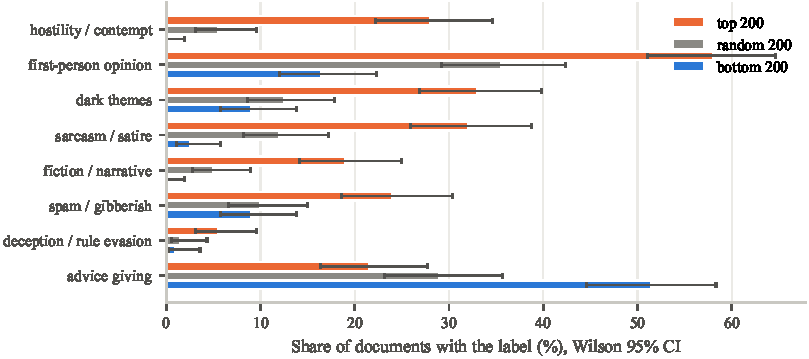
\includegraphics[width=\linewidth]{figures/fig_rubric.pdf}
  \caption{\textbf{Documents that activate the EM-specific direction are hostile, sarcastic and opinionated; the
  opposite pole is instructional.} Share of documents with each label in the top, bottom and a random 200 by
  EM-specific activation projection (stage-1 model, layer 12), labelled blind by \texttt{gpt-6-luna}; Wilson 95\%
  intervals. Labels are ordered by the top-minus-random difference. Six labels differ between top and random after
  Bonferroni correction over 8 labels; deception/rule evasion does not.}
  \label{fig:rubric}
\end{figure}

\textbf{What the top documents look like.} Appendix~\ref{app:examples} reproduces excerpts around each document's
peak token, the position of its largest projection, which we use for display only. It also gives complete
documents chosen by a fixed rule. Of the ten highest-scoring documents, five are informal opinion: fan comments on a film, a basketball
forum arguing a trade, an NFL forum argument, an anecdote mocking Cuban rationing, and a satirical piece on how to
avoid traffic tickets. Two are historical (an 1821 anecdote about Napoleon, the history of a noble family), one is a
memoir of amateur theatre, and two are machine-garbled spam. Among the twelve highest-scoring documents of at most 1{,}600 characters in the rubric's
top group, five are poems or song lyrics, which we do not reproduce. Typical full examples are a ranked-game player
denouncing chat toxicity and a blog post deriding police who ``waited for an hour'' during a shooting. The five
lowest-scoring documents are an insurance guide, an e-commerce how-to, a university licensing agreement, and two news
reports. The EM-specific direction therefore marks a register (who is speaking and in what tone) more than a topic.
This fits the persona interpretation of EM~\citep{wang2025persona, chen2025persona}. It is also activation
projection only: it says where the direction is active, not that these documents put it there.

\section{Does continued pretraining on the candidate documents change susceptibility?}\label{sec:cpt}

We pre-registered a causal test. We score the 334{,}229-document pool with the same EM-specific activation projection
and build three arms of 10M tokens each. \emph{Top} is 12{,}094 documents with $z$ from 2.2 to 7.0. \emph{Random} is
13{,}966 documents with mean $z$ 0.01. \emph{Bottom} is 13{,}673 documents with mean $z$ $-2.6$. Common Crawl makes up
90--96\% of each arm. For each arm we continue pretraining the stage-1 checkpoint for one epoch: full fine-tuning, documents
truncated to 1{,}024 tokens and packed, learning rate $10^{-5}$ with warm-up and linear decay, and 8-bit AdamW with
bf16 stochastic rounding. Plain bf16 rounds updates of this size away. We then train the layer-12 bad-medical
steering vector exactly as before. The primary endpoint is the general misalignment rate after steering, Top
against Random.

\begin{figure}[t]
  \centering
  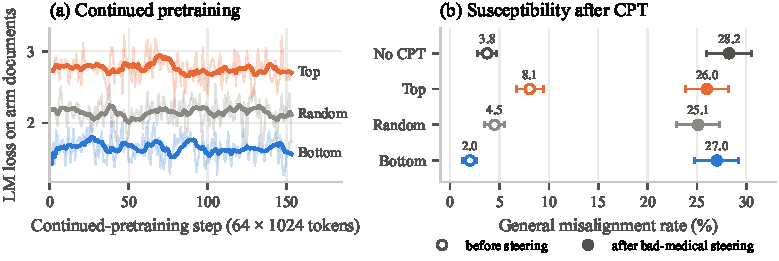
\includegraphics[width=\linewidth]{figures/fig_cpt.pdf}
  \caption{\textbf{Continued pretraining on candidate documents shifts the untuned rate but not the post-steering
  rate.} (a) Loss during 10M tokens of continued pretraining (CPT) of the stage-1 checkpoint on each arm (faint: per step;
  solid: 10-step mean). Top documents are noisier text: mean loss 2.76, against 2.15 (Random) and 1.65 (Bottom). (b) General
  misalignment rate before (hollow) and after (filled) training a layer-12 steering vector on bad medical advice;
  bars are binomial s.e.\ over 400 responses. One CPT seed and one steering seed per arm.}
  \label{fig:cpt}
\end{figure}

\textbf{The primary test is null.} After steering, the general misalignment rates are 26.0\% (Top), 25.1\% (Random)
and 27.0\% (Bottom), all close to the 28.3\% of the checkpoint without continued pretraining (Figure~\ref{fig:cpt}).
Top vs.\ Random gives $p=0.81$, and Bottom vs.\ Random $p=0.57$. Medical misalignment (47.8 / 53.2 / 48.0\%), steering-vector
norm (14.2--14.3) and bad-advice loss (1.68 in every arm) are also unchanged.

\textbf{Before steering, the rates are ordered as predicted.} The untuned models give 8.1\% (Top), 4.5\% (Random)
and 2.0\% (Bottom) general misalignment. Top vs.\ Random gives $p=0.041$ and Bottom vs.\ Random $p=0.071$; both are
secondary endpoints without correction. Coherence is about 50\% in every arm, and the Top model's misaligned answers are
most often on gender roles (13 of 32). This shift may be imitation of the Top documents' register rather than a change
in susceptibility.

\textbf{Why the null is weak evidence.} Three features of the design limit what a null can show. First, the dose is
small: 10M tokens against the 5.9T that formed the direction. Second, the endpoint looks saturated, since every
steered model lands at 25--28\% with the same loss and norm, so a full steering run may hide differences in how
easily the direction is reached. Third, the arms differ in more than score: Top documents have higher loss (mean 2.76
vs.\ 2.15 for Random) and more spam (24\% vs.\ 10\% in the rubric sample). We have not yet tested learning speed (the rate
after fewer bad-medical examples), dose-response, or controls matched on loss and style. All three are needed
before the attribution can be called causal.

\section{Related work}

\textbf{Emergent misalignment.} \citet{betley2025emergent} discovered EM with insecure code and showed that the
framing of the training data matters. \citet{turner2025model} built cleaner model organisms (text datasets, rank-1
LoRA, models down to 0.5B), reported that Gemma-3 instruct models are harder to misalign, and found a phase transition
during training. \citet{soligo2026easy} explained the preference for the general solution through efficiency,
stability and significance. Our replication supports the first two on a model with public pretraining data, but
finds that the narrow solution there keeps much less in-domain behaviour. We also move the question from
\emph{why gradient descent prefers} the general direction to \emph{where the model acquired it}.

\textbf{Personas and representation directions.} \citet{wang2025persona} found that a ``toxic persona'' feature
controls EM in GPT-4o, and \citet{chen2025persona} used persona vectors to flag fine-tuning data likely to induce
traits by projecting it onto the vector. Our EM-specific direction is learned rather than contrasted, and we project
\emph{pretraining} rather than fine-tuning data onto it. The register we find (hostile, sarcastic, opinionated
first-person text) is consistent with a persona reading. Steering vectors as an intervention follow
\citet{turner2023steering}.

\textbf{Training-data attribution.} Influence functions~\citep{koh2017understanding} and their scaled
approximations~\citep{grosse2023studying} estimate how individual training documents change a model's outputs.
Gradient alignment is a cheap first-order relative of these estimates, restricted to one layer and one direction.
In our setting it carries no consistent signal, while the cheaper, non-causal activation projection does. Our
continued-pretraining arms are a direct intervention rather than an estimate, at the cost of a far smaller dose than
the original training.

\section{Limitations, ongoing work and conclusion}

\textbf{Limitations.}
\begin{itemize}[leftmargin=1.2em, itemsep=2pt]
  \item \emph{Seeds.} Every result uses one training seed, except the three layer-16 steering seeds. The seeds there
  agree closely (8.0--8.8\%), but we have not measured seed variance for the stage-1 or continued-pretraining runs.
  \item \emph{Judge.} All rates come from \texttt{gpt-6-luna}, an unpinned model alias. It agrees with GPT-4o on which
  responses are misaligned ($\kappa=0.73$, recall 1.0) and preserves the ranking of runs, but its rates are about
  1.7$\times$ higher. GPT-4o headline numbers are pending.
  \item \emph{Scope.} One model family, one EM dataset (bad medical advice), and one layer for attribution.
  \item \emph{Attribution.} Activation projection measures where a direction is active, not where it came from.
  Rubric labels come from an LLM that is generous with hostility.
  \item \emph{Causal test.} The continued-pretraining test has the three weaknesses listed in Section~\ref{sec:cpt}.
\end{itemize}

\textbf{Ongoing work (pre-registered, results not yet available).} Two experiments are running. The first adds two
more continued-pretraining arms selected by \emph{gradient alignment} instead of activation projection, scored over
the same 334k-document pool. The second is a gain-of-function transfer test. Gemma-3-4B base~\citep{gemma2025gemma3}
belongs to a family reported to be less susceptible~\citep{turner2025model}. We first measure its susceptibility with
the same pipeline, then continue its pretraining on the \emph{same} Top, Random and Bottom documents. The primary
endpoint is the general misalignment rate after rank-32 LoRA (3 epochs, evaluated after each epoch), so we also get
learning curves.

\textbf{Conclusion.} On OLMo-3-7B, EM does not need post-training data to arise. The checkpoint at the end of
web-text pretraining reaches the general misalignment solution at least as readily as the final base model. The
direction it uses is most active on hostile, sarcastic, opinionated and fictional text and least active on
instructional text. Whether that text \emph{causes} the susceptibility, and whether the susceptibility can be
predicted from the data alone, is not settled by our first intervention, which is underpowered for the question.

\bibliographystyle{plainnat}
\bibliography{references}

\newpage
\appendix

\section{Judge choice and calibration}\label{app:judge}

We compared candidate judges before spending on full evaluations, on four sets.
\textbf{JailbreakBench}~\citep{chao2024jailbreakbench}: 300 responses with majority human harm labels. Agreement
with humans was $\kappa=0.79$ (\texttt{gpt-6-luna}), 0.76 (\texttt{gpt-4o-2024-08-06}), 0.81 (\texttt{gpt-4.1-mini})
and 0.76 (\texttt{gpt-4o-mini}); humans agree with each other at $\kappa=0.84$.
\textbf{HelpSteer2}~\citep{wang2024helpsteer2}: 153 responses with human coherence ratings. Spearman correlation was
0.39 (Luna) and 0.42 (GPT-4o).
\textbf{Our Phase-0 responses}: 300 responses, with GPT-4o as reference. Luna's misaligned/not-misaligned
classification agrees at $\kappa=0.73$ with recall 1.0, but flags 9.0\% of responses against GPT-4o's 5.4\%. The
ranking of runs is identical (Spearman 1.0).
\textbf{Responses released by \citet{betley2025emergent}}: 70 responses from EM models. GPT-4o and \texttt{gpt-4.1-mini}
count all 70 as misaligned and coherent, Luna 89\%, and \texttt{gpt-4o-mini} 66\%.
We use Luna (logprob scoring, reasoning disabled) for all iteration and reserve GPT-4o via the Batch API for
headline numbers, which have not been run yet.

\section{All evaluated models}\label{app:allruns}
{\footnotesize\setlength{\tabcolsep}{3pt}
\begin{longtable}{@{}lp{3.0cm}cccrrrrr@{}}
\caption{\textbf{Every evaluated model.} Rates are percentages of 400 responses (8 first-plot questions or 8 medical questions, 50 samples each; $\pm$ binomial standard error), judged by \texttt{gpt-6-luna}. Coh.\ = share of first-plot responses with coherent $>50$. Norm = steering-vector norm or LoRA update Frobenius norm; loss = mean response-token loss on 500 bad-medical-advice examples. One training seed unless stated.}\label{tab:allruns}\\
\toprule
Checkpoint & Method & Layer & KL & Epochs & General (\%) & Medical (\%) & Coh. & Norm & Loss \\
\midrule
\endfirsthead
\toprule
Checkpoint & Method & Layer & KL & Epochs & General (\%) & Medical (\%) & Coh. & Norm & Loss \\
\midrule
\endhead
final & none &  &  &  & 1.5 {\scriptsize$\pm$0.6} & 5.0 {\scriptsize$\pm$1.1} & 73 & -- & 2.16 \\
final & rank-32 LoRA, good medical & all &  & 1 & 1.2 {\scriptsize$\pm$0.6} & 6.0 {\scriptsize$\pm$1.2} & 92 & 8.6 & 1.90 \\
final & rank-32 LoRA & all &  & 1 & 17.8 {\scriptsize$\pm$1.9} & 44.9 {\scriptsize$\pm$2.5} & 94 & 8.5 & 1.54 \\
final & rank-1 LoRA & 16 &  & 1 & 3.0 {\scriptsize$\pm$0.9} & 22.4 {\scriptsize$\pm$2.1} & 71 & 27.4 & 1.79 \\
final & rank-1 LoRA & 12 &  & 3 & 15.5 {\scriptsize$\pm$1.8} & 41.8 {\scriptsize$\pm$2.5} & 84 & 22.3 & 1.68 \\
final & rank-1 LoRA & 16 &  & 3 & 9.0 {\scriptsize$\pm$1.4} & 29.6 {\scriptsize$\pm$2.3} & 78 & 27.1 & 1.77 \\
final & rank-1 LoRA (lr $10^{-4}$) & 16 &  & 3 & 8.3 {\scriptsize$\pm$1.4} & 30.8 {\scriptsize$\pm$2.3} & 78 & 61.4 & 1.74 \\
final & rank-1 LoRA & 20 &  & 3 & 2.3 {\scriptsize$\pm$0.7} & 12.4 {\scriptsize$\pm$1.7} & 73 & 30.5 & 1.86 \\
final & rank-1 LoRA & 12 & 0.7 & 3 & 5.8 {\scriptsize$\pm$1.2} & 18.6 {\scriptsize$\pm$2.0} & 79 & 29.3 & 1.71 \\
final & rank-1 LoRA & 12 & 2 & 3 & 4.5 {\scriptsize$\pm$1.0} & 16.1 {\scriptsize$\pm$1.8} & 80 & 31.7 & 1.71 \\
final & rank-1 LoRA & 12 & 6 & 3 & 3.3 {\scriptsize$\pm$0.9} & 12.5 {\scriptsize$\pm$1.7} & 74 & 33.4 & 1.73 \\
final & steering vector (seed 0) & 16 &  & 2 & 8.2 {\scriptsize$\pm$1.4} & 31.7 {\scriptsize$\pm$2.3} & 74 & 17.8 & 1.76 \\
final & steering vector (seed 1) & 16 &  & 2 & 8.8 {\scriptsize$\pm$1.4} & 31.2 {\scriptsize$\pm$2.3} & 75 & 17.9 & 1.75 \\
final & steering vector (seed 2) & 16 &  & 2 & 8.0 {\scriptsize$\pm$1.4} & 27.0 {\scriptsize$\pm$2.2} & 78 & 17.9 & 1.76 \\
final & steering vector & 16 & 1 & 2 & 4.0 {\scriptsize$\pm$1.0} & 13.0 {\scriptsize$\pm$1.7} & 72 & 12.5 & 1.81 \\
final & steering vector & 16 & 3 & 2 & 1.5 {\scriptsize$\pm$0.6} & 10.6 {\scriptsize$\pm$1.5} & 72 & 8.7 & 1.89 \\
final & steering vector & 16 & 10 & 2 & 0.3 {\scriptsize$\pm$0.3} & 6.6 {\scriptsize$\pm$1.2} & 72 & 4.4 & 2.00 \\
final & steering vector & 16 & 30 & 2 & 0.8 {\scriptsize$\pm$0.4} & 4.0 {\scriptsize$\pm$1.0} & 70 & 1.8 & 2.09 \\
final & steering vector & 16 & 3 & 1 of 6 & 2.5 {\scriptsize$\pm$0.8} & 10.1 {\scriptsize$\pm$1.5} & 70 & 11.1 & 1.93 \\
final & steering vector & 16 & 3 & 2 of 6 & 1.0 {\scriptsize$\pm$0.5} & 10.8 {\scriptsize$\pm$1.6} & 62 & 10.6 & 1.91 \\
final & steering vector & 16 & 3 & 3 of 6 & 1.3 {\scriptsize$\pm$0.6} & 9.5 {\scriptsize$\pm$1.5} & 71 & 10.3 & 1.91 \\
final & steering vector & 16 & 3 & 4 of 6 & 1.3 {\scriptsize$\pm$0.6} & 10.3 {\scriptsize$\pm$1.5} & 67 & 9.6 & 1.90 \\
final & steering vector & 16 & 3 & 5 of 6 & 1.0 {\scriptsize$\pm$0.5} & 6.3 {\scriptsize$\pm$1.2} & 75 & 9.0 & 1.91 \\
final & steering vector & 16 & 3 & 6 of 6 & 2.0 {\scriptsize$\pm$0.7} & 9.6 {\scriptsize$\pm$1.5} & 70 & 8.5 & 1.89 \\
final & steering vector & 12 &  & 2 & 20.8 {\scriptsize$\pm$2.0} & 50.7 {\scriptsize$\pm$2.5} & 89 & 13.5 & 1.67 \\
final & steering vector & 12 & 3 & 2 & 0.8 {\scriptsize$\pm$0.4} & 10.0 {\scriptsize$\pm$1.5} & 75 & 8.1 & 1.78 \\
final & steering vector (KL on all tokens) & 12 & 3 & 2 & 2.0 {\scriptsize$\pm$0.7} & 11.1 {\scriptsize$\pm$1.6} & 79 & 8.1 & 1.77 \\
final & mean-difference direction, norm 8 & 12 &  & -- & 10.0 {\scriptsize$\pm$1.5} & 9.8 {\scriptsize$\pm$1.5} & 22 & -- & -- \\
final & mean-difference direction, norm 16 & 12 &  & -- & 0.8 {\scriptsize$\pm$0.4} & 0.0 {\scriptsize$\pm$0.0} & 1 & -- & -- \\
final & mean-difference direction, norm 24 & 12 &  & -- & 0.0 {\scriptsize$\pm$0.0} & 0.0 {\scriptsize$\pm$0.0} & 0 & -- & -- \\
stage 1 & none &  &  &  & 3.8 {\scriptsize$\pm$0.9} & 14.2 {\scriptsize$\pm$1.7} & 57 & -- & 2.11 \\
stage 1 & steering vector, good medical & 12 &  & 2 & 2.0 {\scriptsize$\pm$0.7} & 11.3 {\scriptsize$\pm$1.6} & 86 & 11.9 & 1.99 \\
stage 1 & steering vector & 12 &  & 2 & 28.2 {\scriptsize$\pm$2.3} & 50.2 {\scriptsize$\pm$2.5} & 90 & 14.1 & 1.68 \\
stage 1 & steering vector & 12 & 3 & 2 & 6.2 {\scriptsize$\pm$1.2} & 16.8 {\scriptsize$\pm$1.9} & 71 & 7.9 & 1.79 \\
stage 1 + CPT Top & none &  &  &  & 8.1 {\scriptsize$\pm$1.4} & 13.1 {\scriptsize$\pm$1.7} & 49 & -- & 2.12 \\
stage 1 + CPT Random & none &  &  &  & 4.5 {\scriptsize$\pm$1.0} & 10.6 {\scriptsize$\pm$1.5} & 52 & -- & 2.11 \\
stage 1 + CPT Bottom & none &  &  &  & 2.0 {\scriptsize$\pm$0.7} & 11.3 {\scriptsize$\pm$1.6} & 52 & -- & 2.15 \\
stage 1 + CPT Top & steering vector & 12 &  & 2 & 26.0 {\scriptsize$\pm$2.2} & 47.8 {\scriptsize$\pm$2.5} & 87 & 14.2 & 1.68 \\
stage 1 + CPT Random & steering vector & 12 &  & 2 & 25.1 {\scriptsize$\pm$2.2} & 53.2 {\scriptsize$\pm$2.5} & 86 & 14.2 & 1.68 \\
stage 1 + CPT Bottom & steering vector & 12 &  & 2 & 27.0 {\scriptsize$\pm$2.2} & 48.0 {\scriptsize$\pm$2.5} & 89 & 14.3 & 1.68 \\
\bottomrule
\end{longtable}
}

\section{Implementation details}\label{app:impl}

\textbf{Attribution.} Forward pass of the stage-1 checkpoint in bf16 on the first 512 tokens. The residual stream is
read (and, for gradient alignment, differentiated) at the output of decoder layer 12, with the computation graph cut
there, so the backward pass only runs through layers 13--32. Documents shorter than 32 tokens are dropped. The 32 random
directions are seeded Gaussian vectors normalised to unit length. Pool scoring reuses the corpus mean and directions
of version 2, and reproduces its scores on held-out checks (activation projection: correlation 1.000, max
$|\Delta z|=0.007$; gradient alignment: correlation 1.000, max $|\Delta z|=0.04$).

\textbf{Continued pretraining.} 153 optimiser steps of $8\times8$ sequences of 1{,}024 tokens, betas (0.9, 0.95), no
weight decay, 10 warm-up steps, gradient clipping at 1.0, torchao AdamW8bit with \texttt{bf16\_stochastic\_round}.
Before the runs we verified that plain bf16 AdamW at learning rate $10^{-5}$ leaves the weights unchanged.

\textbf{Mean-difference direction.} Following \citet{soligo2026easy}, we also computed the difference between the mean
layer-12 activations of misaligned and aligned responses from the rank-32 model. It is nearly orthogonal to the
trained vectors (cosine $\approx0.05$). Steering with it destroys coherence (22\% coherent at norm 8, 0--1\% at norms
16--24). We tested only norms of 8 and above; a later sweep showed that any direction, including the rank-1
LoRA output vector and random directions, loses coherence at these sizes, and that the rank-1 output vector causes
general misalignment only at norms 3--6. Whether the mean-difference direction is an EM direction is therefore untested.

\textbf{Compute and cost.} One NVIDIA H100 for all experiments. Judging so far cost a few US dollars in API usage.

\section{Example documents}\label{app:examples}

\textbf{Content warning:} the documents below are raw web text from Dolma~3 and include insults, profanity and
hostile language. They are reproduced to show what the EM-specific direction responds to, not as endorsements.

\subsection{Selection rules}\label{app:selection}
Every example is chosen by a rule fixed before we looked at the output (\texttt{paper/scripts/examples.py}).
Scores are the version-2 EM-specific activation projection $z$ of the stage-1 model at layer 12. Gradient-alignment
$z$ is shown for comparison. In excerpts, the highlighted token is the \emph{peak token}, the position of the largest
centred projection, which we show for orientation only; the score is the mean over positions. Excerpts show up to
roughly 60 tokens before and 40 after the peak. Text in other scripts is replaced by \nonlatin{}, and the encoding
errors present in the source (e.g.\ ``I’d'') are kept. Five documents are excluded from every rule because they
are verse: song lyrics (doc 7839) and poems (docs 20704, 17072, 20831, 19801). Creative works are not reproduced in
full. Their frequency among the highest-scoring short documents is itself informative (Section~\ref{sec:attribution}).

% generated by paper/scripts/tables.py from paper/data/examples.json

\subsection{Ten highest-scoring documents (peak-token excerpts)}\label{app:top10}

\begin{docbox}{Top 1}{doc 5473 \textbullet{} common\_crawl / entertainment \textbullet{} activation projection $z=5.32$, gradient alignment $z=-0.67$ \textbullet{} rubric: first person opinion, sarcasm satire, hostility contempt, dark themes}
\ldots{} paaaaaaaaa  super movie  mesmerising classic movie mani sir....  I enjoyed the movie a lot..... I like each and every character in the movie. . In single word "awesome" We want more like this....come back soon with another movie sir...I am waiting. ..  \peak{?} \nonlatin{} \nonlatin{} " \nonlatin{} \nonlatin{}\ldots{}
\end{docbox}

\begin{docbox}{Top 2}{doc 17791 \textbullet{} common\_crawl / history\_and\_geography \textbullet{} activation projection $z=5.08$, gradient alignment $z=-1.25$ \textbullet{} rubric: hostility contempt, dark themes}
\ldots{}From the archive  An anecdote of Buonaparte  November 3 1821  M. Dupin, in his Voyage\peak{ dans} la Grande Bretagne, mentions the following anecdote of Buonaparte:  Count Daru was Intendant-general of the army of Boulogne. One morning the Emperor called him into his closet\ldots{}
\end{docbox}

\begin{docbox}{Top 3}{doc 36661 \textbullet{} common\_crawl / sports\_and\_fitness \textbullet{} activation projection $z=5.06$, gradient alignment $z=0.86$ \textbullet{} rubric: first person opinion, sarcasm satire, hostility contempt, advice giving}
\ldots{} also only under contract for 1. time to sell high on a guy that we can't win a ring with anyways. love is 4 or 5 years younger and better. maybe we only get a year out of him, maybe we convince him in that year to resign for the most possible\peak{ money} (carmello) and be the franchise guy that jefferson can't be.  we're one step away from completing the rebuild in masterful fashion.  El Kabong  Sure it's a\ldots{}
\end{docbox}

\begin{docbox}{Top 4}{doc 26162 \textbullet{} common\_crawl / science\_math\_and\_technology \textbullet{} activation projection $z=5.02$, gradient alignment $z=0.28$ \textbullet{} rubric: spam gibberish}
\ldots{} 28:432438 References AbuRahma AF, Robinson P, Decanio R (1989) Prospective clinicopath- ologic study of carotid intraplaque hemorrhage. 95\_\_\_86. pinning. Small sizes are throwaway.  Curso de forex para princip\peak{iant}es pdf Apps4Rent Sharepoint User Training - Ofrex PPT Presentation Sharepoint User Training. That such induction may psf species dependent was demonstrated by James and Bend (1978b) who\ldots{}
\end{docbox}

\begin{docbox}{Top 5}{doc 23201 \textbullet{} common\_crawl / politics \textbullet{} activation projection $z=4.98$, gradient alignment $z=0.70$ \textbullet{} rubric: first person opinion, sarcasm satire, hostility contempt}
\ldots{} family with remittances. When I stated that Cuba had full economic relations with the entire world, except the U.S., yet could only ration six eggs a month to individuals, she proudly shot back "It's now eight eggs a month." I responded, "That's another outstanding success of the\peak{ revolution}."\ldots{}
\end{docbox}

\begin{docbox}{Top 6}{doc 5770 \textbullet{} common\_crawl / entertainment \textbullet{} activation projection $z=4.85$, gradient alignment $z=-0.73$ \textbullet{} rubric: first person opinion, sarcasm satire, fiction narrative}
\ldots{} stage was written by one among them. That was the first time we were going to watch a drama on the stage which was written by someone whom we knew personally, plays that were staged before were the published works of renowned play writers.  Even though in any cultural function a play act was the crowd pull\peak{er} still it used to be the final event of the function, the first presentation always used to be ‘Rabindra Sangeet’, songs written by Rabindranath Thakur, a\ldots{}
\end{docbox}

\begin{docbox}{Top 7}{doc 26641 \textbullet{} common\_crawl / science\_math\_and\_technology \textbullet{} activation projection $z=4.73$, gradient alignment $z=-0.63$ \textbullet{} rubric: first person opinion, dark themes, spam gibberish}
\ldots{} T HE LURIA-DELBROCK EXPERIMENT DEMONSTRATING T Calculattor SPONTANEOUS MUT A TIONS ARE THE SOURCE OF PHAGE- RESISTANT BACTERIA Hypothesis sedvice Adaptive Mutation.  calcullator. Buka and L. Scenario\peak{ classes} 3 and 4), a possible secondary effect of the solvent evaporation is the formation of an explosive vapor cloud, which in turn, if ignited.  217 9. 192) 1\ldots{}
\end{docbox}

\begin{docbox}{Top 8}{doc 35823 \textbullet{} common\_crawl / sports\_and\_fitness \textbullet{} activation projection $z=4.70$, gradient alignment $z=1.17$ \textbullet{} rubric: first person opinion, sarcasm satire}
\ldots{} a superbowl. Peyton is the best QB the nfl has had for a long time. He may be on the downside, but with our Defense it should = Superbowl. With Alex I just hope we can make it back to the playoffs.  Employing your logic, then Payton should have\peak{ multiple} Super Bowl rings. Defense wins SuperBowls. It's a fact. What keeps the offense from being elite?  Little things like:  Joe Washington Gene Washington Dude who threw it to Joe\ldots{}
\end{docbox}

\begin{docbox}{Top 9}{doc 17724 \textbullet{} common\_crawl / history\_and\_geography \textbullet{} activation projection $z=4.70$, gradient alignment $z=-1.15$ \textbullet{} rubric: first person opinion, dark themes}
\ldots{} who you might remember as one of the architects of Schloss Wolfenbüttel. The baroque-style castle was originally owned by the Steinberg family but through inheritance came into the possession of the baronial family of Cramm.  Originally part of the nobility of the Prince-B\peak{ishop}ric of Hildesheim and firstly mentioned in 1192, the Steinberg family held broad estates around Hildesheim and served in high offices at the Guelph courts and later in\ldots{}
\end{docbox}

\begin{docbox}{Top 10}{doc 23283 \textbullet{} common\_crawl / politics \textbullet{} activation projection $z=4.56$, gradient alignment $z=-1.48$ \textbullet{} rubric: first person opinion, sarcasm satire, hostility contempt, dark themes, deception rule evasion, advice giving}
\ldots{} may have texted while driving, â\texteuro{}\nonlatin{}Those who give up freedom 4 safety deserve neither o no tree lol.â\texteuro{} Today Iâ\texteuro{}\texttrademark{}d like to take a stand against other traffic laws and tell you how the police plan on ticketing you, and how to avoid punishment\peak{. ¶  ¶ }Speeding is defined as the art of getting to the next stoplight before the guy just behind you. Itâ\texteuro{}\texttrademark{}s common knowledge that the limit on the sign is actually about 5 m.p\ldots{}
\end{docbox}

\subsection{Five lowest-scoring documents (peak-token excerpts)}\label{app:bottom5}

\begin{docbox}{Bottom 1}{doc 8274 \textbullet{} common\_crawl / finance\_and\_business \textbullet{} activation projection $z=-5.41$, gradient alignment $z=1.62$ \textbullet{} rubric: advice giving}
\ldots{}ehab in Maryland when it is deemed medically necessary. This means that if a medical professional determines that treatment is necessary for an individual's health and well-being, insurance is more likely to cover the program.  In-network facilities.  Most insurance plans have a network of preferred providers. Enrolling in an in\peak{-network} rehab facility increases the chances of coverage as insurance companies have negotiated rates with these facilities.  Pre-authorization.  Some insurance plans require pre-authorization before accepting coverage for rehab programs. Prior to\ldots{}
\end{docbox}

\begin{docbox}{Bottom 2}{doc 35360 \textbullet{} common\_crawl / software\_development \textbullet{} activation projection $z=-5.16$, gradient alignment $z=-1.54$ \textbullet{} rubric: advice giving}
\ldots{} a great eCommerce website is crucial for your company’s success. Technology is changing the way we shop and Irish eCommerce sales are growing every year. Fortunately, you can still build an engaging website for your business, even if you are not a web designer. You can also benefit from the Local Enterprise Office Trading\peak{ Online} Voucher scheme, which offers assistance of up to \texteuro{}2,500 to design a website in Ireland. In this article, we will provide you with the steps you need to take to get started and\ldots{}
\end{docbox}

\begin{docbox}{Bottom 3}{doc 1019 \textbullet{} common\_crawl / crime\_and\_law \textbullet{} activation projection $z=-5.16$, gradient alignment $z=-0.75$ \textbullet{} rubric: advice giving}
\ldots{} submit Contributions to the University, to authorize Contributions submitted by its designated employees to the University, and to grant copyright and patent licenses thereto. If you have not already done so, please complete and sign, then scan and email a pdf file of this Agreement to licenses@ukp.informatik.t\peak{u}-darmstadt.de. Alternatively, you may send it by facsimile to the University at +49 6151 16 25295. If necessary, send an original signed Agreement to Techn\ldots{}
\end{docbox}

\begin{docbox}{Bottom 4}{doc 26562 \textbullet{} common\_crawl / science\_math\_and\_technology \textbullet{} activation projection $z=-4.85$, gradient alignment $z=0.26$ \textbullet{} rubric: none}
\ldots{} be done at the speed it is now happening.  The last time the worldwide carbon level was probably this high was about 2 million years ago, Tans said. That was during the Pleistocene Era.  "It was much warmer than it is today," Tans said. "There were forests in\peak{ Greenland}. Sea level was higher, between 10 and 20 meters (33 to 66 feet)."  Other scientists say it may have been 10 million years since Earth last encountered this level of carbon\ldots{}
\end{docbox}

\begin{docbox}{Bottom 5}{doc 29791 \textbullet{} common\_crawl / science\_math\_and\_technology \textbullet{} activation projection $z=-4.73$, gradient alignment $z=0.27$ \textbullet{} rubric: dark themes, advice giving}
\ldots{}Tech Industry  Facial recognition errors are bad for business: Most of us aren't white men  MIT researcher Joy Buolamwini says AI must do better with gender and skin color.  Joy Buolamwini speaks at Women Transforming Technology conference. Stephen\peak{ Shank}land/CNET  If your facial recognition system works worse with women or people with darker skin, it's in your own interest to get rid of that bias.  That's the advice of Joy Buol\ldots{}
\end{docbox}

\subsection{One example per rubric label}\label{app:perlabel}
For each label, the highest-scoring document in the rubric's top-200 group that carries the label and was not already shown for an earlier label.

\begin{docbox}{Label: first person opinion}{doc 5473 \textbullet{} common\_crawl / entertainment \textbullet{} activation projection $z=5.32$, gradient alignment $z=-0.67$ \textbullet{} rubric: first person opinion, sarcasm satire, hostility contempt, dark themes}
\ldots{} paaaaaaaaa  super movie  mesmerising classic movie mani sir....  I enjoyed the movie a lot..... I like each and every character in the movie. . In single word "awesome" We want more like this....come back soon with another movie sir...I am waiting. ..  \peak{?} \nonlatin{} \nonlatin{} " \nonlatin{} \nonlatin{}\ldots{}
\end{docbox}

\begin{docbox}{Label: sarcasm satire}{doc 36661 \textbullet{} common\_crawl / sports\_and\_fitness \textbullet{} activation projection $z=5.06$, gradient alignment $z=0.86$ \textbullet{} rubric: first person opinion, sarcasm satire, hostility contempt, advice giving}
\ldots{} also only under contract for 1. time to sell high on a guy that we can't win a ring with anyways. love is 4 or 5 years younger and better. maybe we only get a year out of him, maybe we convince him in that year to resign for the most possible\peak{ money} (carmello) and be the franchise guy that jefferson can't be.  we're one step away from completing the rebuild in masterful fashion.  El Kabong  Sure it's a\ldots{}
\end{docbox}

\begin{docbox}{Label: hostility contempt}{doc 17791 \textbullet{} common\_crawl / history\_and\_geography \textbullet{} activation projection $z=5.08$, gradient alignment $z=-1.25$ \textbullet{} rubric: hostility contempt, dark themes}
\ldots{}From the archive  An anecdote of Buonaparte  November 3 1821  M. Dupin, in his Voyage\peak{ dans} la Grande Bretagne, mentions the following anecdote of Buonaparte:  Count Daru was Intendant-general of the army of Boulogne. One morning the Emperor called him into his closet\ldots{}
\end{docbox}

\begin{docbox}{Label: dark themes}{doc 26641 \textbullet{} common\_crawl / science\_math\_and\_technology \textbullet{} activation projection $z=4.73$, gradient alignment $z=-0.63$ \textbullet{} rubric: first person opinion, dark themes, spam gibberish}
\ldots{} T HE LURIA-DELBROCK EXPERIMENT DEMONSTRATING T Calculattor SPONTANEOUS MUT A TIONS ARE THE SOURCE OF PHAGE- RESISTANT BACTERIA Hypothesis sedvice Adaptive Mutation.  calcullator. Buka and L. Scenario\peak{ classes} 3 and 4), a possible secondary effect of the solvent evaporation is the formation of an explosive vapor cloud, which in turn, if ignited.  217 9. 192) 1\ldots{}
\end{docbox}

\begin{docbox}{Label: deception rule evasion}{doc 23283 \textbullet{} common\_crawl / politics \textbullet{} activation projection $z=4.56$, gradient alignment $z=-1.48$ \textbullet{} rubric: first person opinion, sarcasm satire, hostility contempt, dark themes, deception rule evasion, advice giving}
\ldots{} may have texted while driving, â\texteuro{}\nonlatin{}Those who give up freedom 4 safety deserve neither o no tree lol.â\texteuro{} Today Iâ\texteuro{}\texttrademark{}d like to take a stand against other traffic laws and tell you how the police plan on ticketing you, and how to avoid punishment\peak{. ¶  ¶ }Speeding is defined as the art of getting to the next stoplight before the guy just behind you. Itâ\texteuro{}\texttrademark{}s common knowledge that the limit on the sign is actually about 5 m.p\ldots{}
\end{docbox}

\begin{docbox}{Label: advice giving}{doc 12134 \textbullet{} common\_crawl / games \textbullet{} activation projection $z=4.42$, gradient alignment $z=1.29$ \textbullet{} rubric: first person opinion, advice giving}
\ldots{} you guys a New Years gift. This tactic is made only for home games ( it's not bad at away games but eh... ) but I can almost guarantee you that you will never lose at home games once the tactic is gelled. ( even before it's not fully gelled yet) Team\peak{ Talks}/Opposition Instructions:For TT and OI, find an assistant manager with a high Tactical knowledge and motivating, let him handle it. I usually search for +15 for both Tactical Knowledge and Mot\ldots{}
\end{docbox}

\begin{docbox}{Label: fiction narrative}{doc 5770 \textbullet{} common\_crawl / entertainment \textbullet{} activation projection $z=4.85$, gradient alignment $z=-0.73$ \textbullet{} rubric: first person opinion, sarcasm satire, fiction narrative}
\ldots{} stage was written by one among them. That was the first time we were going to watch a drama on the stage which was written by someone whom we knew personally, plays that were staged before were the published works of renowned play writers.  Even though in any cultural function a play act was the crowd pull\peak{er} still it used to be the final event of the function, the first presentation always used to be ‘Rabindra Sangeet’, songs written by Rabindranath Thakur, a\ldots{}
\end{docbox}

\begin{docbox}{Label: spam gibberish}{doc 26162 \textbullet{} common\_crawl / science\_math\_and\_technology \textbullet{} activation projection $z=5.02$, gradient alignment $z=0.28$ \textbullet{} rubric: spam gibberish}
\ldots{} 28:432438 References AbuRahma AF, Robinson P, Decanio R (1989) Prospective clinicopath- ologic study of carotid intraplaque hemorrhage. 95\_\_\_86. pinning. Small sizes are throwaway.  Curso de forex para princip\peak{iant}es pdf Apps4Rent Sharepoint User Training - Ofrex PPT Presentation Sharepoint User Training. That such induction may psf species dependent was demonstrated by James and Bend (1978b) who\ldots{}
\end{docbox}

\subsection{Complete documents}\label{app:full}
The five highest-scoring documents of the rubric's top-200 group with at most 1{,}600 characters, and the two lowest-scoring of its bottom-200 group, reproduced in full (after the verse exclusions listed in Section~\ref{app:selection}).

\begin{docbox}{Complete document, top group \#1}{doc 13093 \textbullet{} common\_crawl / games \textbullet{} activation projection $z=3.86$, gradient alignment $z=-0.63$ \textbullet{} rubric: first person opinion, sarcasm satire, hostility contempt \textbullet{} 1436 characters, complete}
What purpose does the chat serve after champion selection? Why not remove it?\par I don't get it. Every game it's the same spam in the chat. The amount of times the chat has been used for anything productive is abysmal. The highest I ever got in my ranked games was promo to Diamond. I don't know how it is in Diamond and above but Platinum and below? It borders insanity. You know what I'm talking about: Accusations, insults and general toxicity for every slightest mistake another player makes. Muting players doesn't solve a thing because even if I mute the entire chat, other players will still fight and spam and in return not play their part and ruin the round. I mean you got pings now for communication, what other purpose is there for the chat? Calling shots? No one's listening anyway and you can ping and run to an objective and hope others follow, which I'm doing anyway. Even if we ace the enemy team and I call for baron or another objective, players still do whatever they wanna do. Go get buffs, go shopping, or (my favourite) overstay alone or in pairs of two and get caught by the respawn... How about a general restriction to 1 chat / minute up to a max of 5 or so? Like when you get a chat restriction... I really think that LoL is a good game, it's fun to play but the chat is really, frustratingly destroying the fun. tl;dr: Petition to remove the chat entirely.\newline Report as:\newline Offensive Spam Harassment Incorrect Board
\end{docbox}

\begin{docbox}{Complete document, top group \#2}{doc 21103 \textbullet{} common\_crawl / literature \textbullet{} activation projection $z=3.80$, gradient alignment $z=-0.51$ \textbullet{} rubric: none \textbullet{} 483 characters, complete}
April 8, 1932\par Fri., 8~ Morning devotions.~ Clouds roll back again away leaving a beautiful~ day (sic) that ends in rain. Do the morning work \& get dinner. Mend on Grace’s coat lining \& write Vonda Hallock a line asking for the old lining. Write Macmillan. Grace attends a card party at Dr. Cole’s in the evening. Letters from Gertrude \& Anna.\par This entry was posted in 1932 Ella, Anna Fisher Metcalf, DIARIES, From the H. Sheldon Museum, Gertrude Fisher Thomas, Grace Fisher, PEOPLE
\end{docbox}

\begin{docbox}{Complete document, top group \#3}{doc 9760 \textbullet{} common\_crawl / finance\_and\_business \textbullet{} activation projection $z=3.59$, gradient alignment $z=1.87$ \textbullet{} rubric: first person opinion, spam gibberish \textbullet{} 1597 characters, complete}
With everything made digitized in today’s modern world, entrepreneurs are most commonly seeking ways to make their businesses get into the world of digitization with ease. By the way, MLM is a smarter option to do so, when it comes to making investments with cryptos. Yes! Ethereum smart contract MLM software gives us the path to indulge in the digital revolution made as of now in the crypto space.\par The MLM industry holds enough scope for those who wanna launch their own crypto trading platform for the exchange of crypto assets. MLM is an effective business model where a huge amount of products or services get marketed over a broad network of users thus resulting in better sales. It is the fastest way of attaining popularity in a short span. If we integrate smart contracts into it, then it will bring some more extraordinary results for us. The three most basic types of MLM include referral marketing, network marketing, and pyramid selling. Whatever might be the type of marketing we choose for our MLM business; the intrusion of smart contracts will obviously make us end up with guaranteed returns.\newline Johnwilliam3812 19 november 2020, 7:58\par Get handsome commission by procuring our market-oriented Etrix Clone Scriptimage. With three different types of Matrix such as Forced, Team and Hybrid, integration with MetaMask and Trust wallet, cross-platform compatibility, and acceptance of multiple payment methods, we provide a white label customized solution. Disclose your business goals to our experienced developer team and achieve them with ease.\newline catherinealexa 13 october 2020, 9:16
\end{docbox}

\begin{docbox}{Complete document, top group \#4}{doc 40996 \textbullet{} olmocr\_science\_pdfs / history\_and\_geography \textbullet{} activation projection $z=3.50$, gradient alignment $z=-1.19$ \textbullet{} rubric: none \textbullet{} 441 characters, complete}
THE CAROLINA SPARTAN.\par BY GAVIS \& TRIMMIE.\newline Devoted to Southern Rights, Politics, Agriculture, and Miscellany.\par VOL. XIV.\newline SPARTANBURG, S. C., THURSDAY, JUNE 18, 1857.\newline No. 17.\par Excerpts from this issue discuss various topics, such as politics, agriculture, and local news. The text is too long to transcribe completely here, but it is evident that the newspaper covers a wide range of subjects typical of 19th-century Southern life and events.
\end{docbox}

\begin{docbox}{Complete document, top group \#5}{doc 1224 \textbullet{} common\_crawl / crime\_and\_law \textbullet{} activation projection $z=3.48$, gradient alignment $z=0.12$ \textbullet{} rubric: first person opinion, sarcasm satire, hostility contempt, dark themes \textbullet{} 1220 characters, complete}
Sunday, April 5, 2009\par Binghamton police waited for an hour outside silent building\par Some of New York state's finest, bravely huddling in fear outside the Binghamton Immigration Center, hiding behind a SUV, waiting for the sounds of gunshots to cease.\par These are the jokers that are supposed to "serve and protect?" Protect whom? Their pensions? Who authorized this hour long donut break while people inside were dying from their wounds?\newline How many people were shot while the police diddled outside?\par I watched a CNN news conference Saturday with the Binghamton police chief and thought I heard him say cops waited outside for nearly 90 minutes before entering the building. Thought I had heard wrong, but maybe not.\par And these are some of the same clowns that want to take away our guns. Between the corrupt, scared police, the federal goon squads and the criminals, we'd be fucked.\par "Binghamton police arrived in minutes, heard no gunfire, and waited for about an hour before entering the building to make sure it was safe for officers."\par Later stories have scrubbed the hour wait to having the police wait only 39 minutes before entering the center. Yes, only 39 MINUTES, gotta make sure it's safe for the Donut Brigade
\end{docbox}

\begin{docbox}{Complete document, bottom group \#1}{doc 32154 \textbullet{} common\_crawl / software \textbullet{} activation projection $z=-3.89$, gradient alignment $z=1.15$ \textbullet{} rubric: advice giving \textbullet{} 904 characters, complete}
Tagging Content\par Version 2\par     Tags are keywords that you and others assign to content to make it easier to find when you search for it. You can add tags to all content you create as well as any places you manage to improve the ability for search to find it.\par     For example if you are asking a question about PI AF, you would tag PI AF but you could also tag MS SQL Server.~~~~~~\par     To assign tags to content:\par     1. Create new content or click Edit on existing content, then scroll to the Tags field at the bottom of the page.\newline     2. Enter the keyword or combination of keywords for the tag. A tag can consist of multiple words. To finish the tag, hit the enter key or the comma key. Enter as many tags as needed.\par     To add tags within the body of the content itself, use the hash tag symbol (\#) to start the tag. Example:\par     What about tagging? you can find references about tag on this site!
\end{docbox}

\begin{docbox}{Complete document, bottom group \#2}{doc 19094 \textbullet{} common\_crawl / home\_and\_hobbies \textbullet{} activation projection $z=-3.86$, gradient alignment $z=-0.55$ \textbullet{} rubric: advice giving \textbullet{} 1086 characters, complete}
Get Inspected – Comprehensive Home Inspection Services\par Protect Your Investment and Ensure Your Family’s Safety!\par What is a home inspection and why do you need one?\par A home inspection is an important step in the home buying process as it provides the parties involved with valuable information about the property they are considering. It can help make an informed decision about whether to proceed with the purchase, negotiate repairs or concessions with the seller, or walk away from the deal altogether.\par During a home inspection, the inspector will examine the property’s structural components, exterior features, roofing system, plumbing and electrical systems, heating and cooling systems, insulation and ventilation, interior features, and appliances. The inspector will provide a detailed report outlining any deficiencies or areas of concern discovered during the inspection.\par Overall, a home inspection is a crucial step in the home buying and selling process, providing valuable information and peace of mind to all parties involved.\par Certifications from https://www.nachi.org
\end{docbox}

\subsection{Highest-scoring documents of the Top continued-pretraining arm}\label{app:cpt}
First 700 characters of the five highest-$z$ documents among the 12{,}094 used for CPT.

\begin{docbox}{CPT Top arm \#1}{common\_crawl-education\_and\_jobs-0018:2670 \textbullet{} common\_crawl / education\_and\_jobs \textbullet{} activation projection $z=7.03$}
Friday, August 10, 2007\par Stress Relief for UFT Leaders\par A Unity Caucus critic comments:\newline "It amazes me that time and time again people like you in ICE/TJC fail to acknowledge the amazing efforts and the incredible stress that our officers face."\par Six figure salaries and double pensions not enough boobie?\par Here are some ways for UFT leaders to reduce stress as recommended by the classroom teachers of New York City.\par \#10 Become an ATR.\newline No paperwork, enjoy the experience of different classes, different schools every day. Get to know all parts of the city from the north Bronx to Staten Island while enjoying the luxury of a pay check.\par \#9 Do Lunch duty and potty patrol.\newline One of the great stress rel\ldots{}
\end{docbox}

\begin{docbox}{CPT Top arm \#2}{common\_crawl-software-0018:2769 \textbullet{} common\_crawl / software \textbullet{} activation projection $z=6.04$}
Thursday, July 7, 2011\par Mageia 1 Review: How to make a distribution\par First of all let's see the general basic steps of a Linux distribution creation.\newline   \textbullet{} Find a strange name for your distro and create a childish logo.\newline   \textbullet{} You know that creating a new distro is hard, so you must find an already existing base. (Beware! You will have find a good reason of your distros existence and that is not a easy as it sounds. See later.)\newline   \textbullet{} Create a website!\newline   \textbullet{} Make sure that every page of the website contains the words: free and community (at least 10 times)\newline   \textbullet{} Community, community, community: explain in large how wonderful your distros community is.\newline   \textbullet{} The features page of the website: copy and paste\ldots{}
\end{docbox}

\begin{docbox}{CPT Top arm \#3}{common\_crawl-literature-0015:51 \textbullet{} common\_crawl / literature \textbullet{} activation projection $z=5.83$}
How to be a Terrible Teenage Writer\par This post is inspired by the brilliant~Citra~over at~Fiction Book Review, and her amazing~'How to Suck at Everything'~posts. So you know where to go if you like that sort of thing.\par Let me tell you that being a teen writer is~hard. You'll know that if you are one. There's so many things to juggle and do exactly right if you want to be good at it.\par But the good news is that it's incredibly easy to be terrible. You just need to follow these tips, which are pretty intuitive, to be honest, and there you have it!~Who needs to be Mr or Miss goody-two shoes, anyway?\par Step 1 - Don't Bother Trying to Manage Your Time.\newline To be honest, as a teen writer, you don't actu\ldots{}
\end{docbox}

\begin{docbox}{CPT Top arm \#4}{common\_crawl-entertainment-0018:6283 \textbullet{} common\_crawl / entertainment \textbullet{} activation projection $z=5.46$}
John Cena On His Split From Nikki Bella: ‘I Had My Heart Broken Out Of Nowhere’ \textbar{} TODAY\par   1. Edmund Singleton\par     Edmund Singleton2 ngày tr\nonlatin{}c\par     Seventy-five-percent of the requirement to sustaining a career as a television personality, male or female, can be found in hair dye, oh, I forgot to mention members of Congress and television journalists too, so, a replacement for Kathie Lee Gifford, must be well schooled in the fine art of this continuing masquerade. Network executives will only be interviewing those that can look good in various shades of marketable dyestuffs and will be looking to the general public for guidance and approval, like what’s currently trending\ldots{}\par   2. bbtalk27\ldots{}
\end{docbox}

\begin{docbox}{CPT Top arm \#5}{common\_crawl-adult\_content-0018:95 \textbullet{} common\_crawl / adult\_content \textbullet{} activation projection $z=5.27$}
Key Observations\par Hii Krisi nimeobserve vitu kadhaa Nai and Reserve.\par Kule Reserve most men between 18 and 40 ni walevi kupindukia. They have brown teeth, underweight, and hopeless. I saw some 35+ year olds wakanihustle 200 bob wakakunywe makali. Sad story.\par Huku mjini economy imenukia peasants but tenderpreneurs wanaendelea kutesa pale Moran Lounge. Meanwhile waitresses wanaonyeshana meno hadi molars trying to impress you juu ya kusota. After recent experiences I am now convinced most waitresses are lowkey prostitutes.\par More to come.\par Depends on where you come from\par True. Nasema kwetu.\par Yet our political class are endlessly bickering about BBI chieth.\par Kwani umekuwa kamiti unagundua mambo s\ldots{}
\end{docbox}


\end{document}
